\documentclass{sig-alternate}
\usepackage{txfonts}
\usepackage{ifpdf}
\usepackage{amsmath}
\usepackage{mathrsfs}
\usepackage{amsfonts}
\usepackage{subfigure}
\usepackage{graphicx}
\usepackage{latexsym}
\usepackage{multirow}
\usepackage{microtype}
\usepackage{algorithm}
\usepackage{paralist}
\usepackage[sort]{cite}
\usepackage[pdfborder={0 0 0},plainpages,pdfpagelabels=false]{hyperref}

\setlength{\paperheight}{11in}
\setlength{\paperwidth}{8.5in}

\newtheorem{theorem}{Theorem}
\newtheorem{proposition}[theorem]{Proposition}
\newtheorem{claim}[theorem]{Claim}
\newtheorem{lem}[theorem]{Lemma}
\newtheorem{terminology}[theorem]{Terminology}
\newtheorem{corollary}[theorem]{Corollary}
\newtheorem{observation}[theorem]{Observation}
\newtheorem{problem}[theorem]{Problem}


\newtheorem{defi}[theorem]{Definition}
\newtheorem{exa}[theorem]{Example}

% QED symbol at the end of definitions and examples
\newif\ifqedwritten
\newenvironment{definition}[1][]{\begin{defi}[#1]\upshape\qedwrittenfalse}{\qedhere\end{defi}}
\newenvironment{example}{\begin{exa}\upshape\qedwrittenfalse}{\qedhere\end{exa}}
\newcommand{\qedhere}{\ifqedwritten\else\ifmmode\tag*{\qed}\else\hfill\qed\fi\global\qedwrittentrue\fi}

\newcommand{\topk}{\mbox{top-$k$}}
\newcommand{\Topk}{\mbox{Top-$k$}}
\newcommand{\topkm}{\mbox{top-$k$,$m$}}
\newcommand{\Topkm}{\mbox{Top-$k$,$m$}}

\renewcommand{\leq}{\leqslant}
\renewcommand{\geq}{\geqslant}

% More tolerant setting for floats -- more compactness
\renewcommand\floatpagefraction{.9}
\renewcommand\topfraction{.9}
\renewcommand\bottomfraction{.9}
\renewcommand\textfraction{.1}
\setcounter{totalnumber}{50}
\setcounter{topnumber}{50}
\setcounter{bottomnumber}{50}

\renewcommand{\textfloatsep}{1em}
\renewcommand{\dbltextfloatsep}{1em}

%%%%%%%%%%%%%%%  Magic for tighter spacing around theorem-like environments
\makeatletter
\def\@begintheorem#1#2{%
    \vspace{-3pt}
    \parskip -1pt
    \trivlist
    \item[%
        \hskip 10\p@
        \hskip \labelsep
        {{\sc #1}\hskip 5\p@\relax#2.}%
    ]
    \it
}
\let\old@endtheorem\@endtheorem
\def\@endtheorem{\old@endtheorem\vspace{-8pt}}
\makeatother

\begin{document}

%\conferenceinfo{SIGMOD '12,} {May 20--24, 2012, Scottsdale, Arizona, USA.}
%\CopyrightYear{2012}
%\crdata{978-1-4503-1247-9/12/05}
%\clubpenalty=10000
%\widowpenalty = 10000


\title{Exact and Approximate String Joins with Taxonomy}

%\numberofauthors{5}

\author{
%\alignauthor{Jiaheng Lu  \\
%       \affaddr{$^{\dag}$ School of Information and DEKE, MOE, Renmin
%University of China; Beijing, China}\\
%       \email{\{jiahenglu\}@ruc.edu.cn,  pierre@senellart.com}
%}
}


%For example, in XML keyword query refinement, each
%keyword is associated with a set of alternative terms.  Each term is
%associated with an inverted list containing the occurrences and the
%weights of the corresponding elements in the XML database. The
%\topkm{} queries return top-$k$ refined keyword combinations
%according to the corresponding \mbox{top-$m$} search results of keyword
%queries. In general, \topkm{} queries are useful in scenarios
%where the problem of selecting \emph{combinations
%of attributes} associated with ranked inverted lists naturally occurs.
%Applications range


\maketitle

\begin{abstract}

A string join finds all string pairs between two input string collections. It is an essential operation in
many applications, such as data integration and data cleansing. This paper investigates a novel challenge to integrate taxonomy into string joins. In general, the taxonomy presents a general-purpose strategy to improve the accuracy of string joins by enriching data with semantics-based knowledge  (i.e., a set of IS-A hierarchies). For example,  ``\textsf{California}'' is a state of ``\textsf{U.S.}'' in a geographical taxonomy.

In this work, we study both exact-join and approximate-join cases with taxonomy. Exact joins mean that two strings have the exact IS-A relation, while approximate joins extend the existing similarity functions to capture the IS-A relations against part of strings. Although approximate string joins were studied without taxonomy, we encounter new  challenges here: two strings, which are similar with a taxonomy-based similarity function, may not share any common token. That means, the existing signature-based filtering strategy do not work any more.  In this paper, we propose a set of novel algorithms and filtering strategies for both exact-joins and approximate-joins. The technique relies on the insight that two strings are similar only if they share certain number of common tokens and/or they have IS-A relations in the taxonomy.  The extensive performance evaluation shows that our algorithms can utilize the taxonomy to improve the effectiveness of string joins  and  scale very well with important parameters like data size and taxonomy size.


\end{abstract}

%\category{H.2.4}{Database Management}{Systems}[Query processing]
%\category{H.3.3}{Database Management}{Information Search and
%Retrieval}[Search process]

%\terms{Algorithms, Experimentation, Performance, Theory}

%\keywords{keyword search, package search, top-$k$ querying}

\section{Introduction}

\begin{figure}[t]
\centering
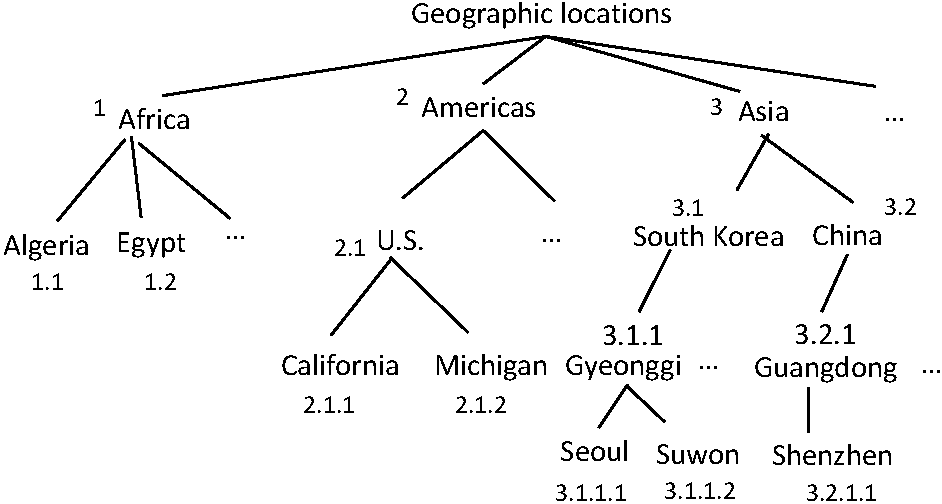
\includegraphics[width=0.45\textwidth]{figures/taxonomylabels}
 \caption{An example of geographical taxonomy with labels}
\label{fig:toytaxonomyexample}
\end{figure}


A string join, which finds all equivalent string pairs between two input collections, is an essential operation in many applications, such as  data integration \cite{conf/sigmod/Sarawagi04}, data cleansing \cite{conf/vldb/ArasuGK06,journals/www/LiJM06} and record linkage \cite{books/Winkler99}. In practice, the same object/entity may have different representations  due to a variety of reasons such as misspellings
caused by typographic errors and different formatting conventions including synonyms, abbreviations and acronyms. Hence, it is important to support approximate string joins for reconciling different
representations of an entity. A large number of  similarity functions such as Levenshtein distance~\cite{conf/sigmod/WangLF12},
Hamming distance~\cite{conf/spire/Kondrak05}, Episode
distance~\cite{conf/ijcai/CohenRF03}, Cosine
metric~\cite{journals/ipm/SaltonB88}, Jaccard
Coefficient~\cite{conf/icde/ChaudhuriGK06,conf/icde/LiLL08}, JaccT \cite{conf/icde/ArasuCK08} and Synonym-based similarity \cite{conf/sigmod/LuLWLW13} have been proposed in the literature. It is well known
that no single similarity function is universally applicable
across all domains and scenarios.

In this paper, we investigate a novel problem to exploit taxonomy with string similarity joins. In principle, the taxonomy presents a general purpose strategy to improve the accuracy of string joins by enriching data with semantics-based knowledge. Taxonomies are sets of IS-A hierarchies, which identify the relations between different concepts. The IS-A relationship
is a transitive closure of the concept-instance relationship.
For example, if ``\textsf{kitten}'' is an instance of ``\textsf{cat}'', and
``\textsf{cat}'' is an instance of ``\textsf{pet}'', then ``\textsf{kitten}'' is an instance
of ``\textsf{pet}''. If we treat each term as a node, and create
for each (concept, instance) pair, an edge from the concept
to the instance, then we can think of the taxonomy as a tree or forest. For any node that representing a term,
the IS-A relation could be any descendant of it in the tree. Figure
\ref{fig:toytaxonomyexample} gives a toy example of a geographical taxonomy tree.

Based on the taxonomy,  the similarity of two strings can be measured in a \textit{semantic} way. For example, consider two pairs (\textsf{Los Angles}, \textsf{Cupertino}) and (\textsf{Los Angles}, \textsf{Seoul}). Intuitively, the similarity between \textsf{Los Angles} and \textsf{Cupertino} should be greater than that between \textsf{Los Angles} and \textsf{Seoul}, because the formers are two cities in the same country and the same state. To quantify the similarity, one method is to calculate the longest common prefixes (LCP) between two strings against the taxonomy. Thus, based on Figure \ref{fig:toytaxonomyexample}, LCP(\textsf{Los Angles}, \textsf{Cupertino})= 4, but (\textsf{Los Angles}, \textsf{Seoul})=1. Clearly the similarity between \textsf{Los Angles} and \textsf{Cupertino} is greater than that between \textsf{Los Angles} and \textsf{Seoul}.


\begin{figure}[t]
\centering
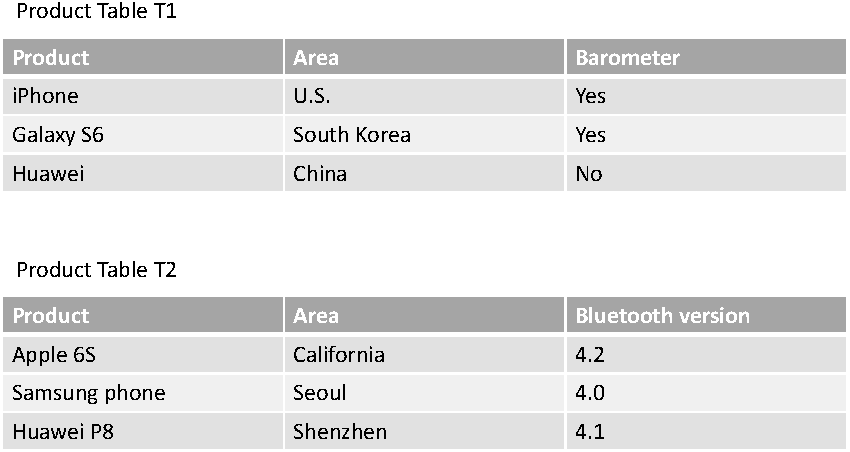
\includegraphics[width=0.45\textwidth]{figures/productexample}
 \caption{Two tables for data integration}
\label{fig:twotables}
\end{figure}

We give several applications to shed light on the importance of the  string similarity matching with taxonomy on databases.

\begin{itemize}
  \item \textbf{Data Integration} ~ Data integration involves combining data residing in different sources. Taxonomy is quite useful to  discover the relations of various objects. For example, consider two tables in Figure \ref{fig:twotables}. In order to correctly perform the integration between two tables, the system needs to know hat ``\textsf{Apple 6s is a model of iphone}'' and ``\textsf{Cupertino is a city in US}'', and etc. A join mechanism that can utilize such taxonomy knowledge may help users to discover more relevant records and thus to improve the effectiveness of data integration.
  \item \textbf{Data mining} ~ Term classification and term clustering are two important tasks in data mining. A new similarity measure that can find the IS-A relations between terms is beneficial to term classification and clustering algorithms to improve their accuracies \cite{journals/dke/CaglieroG13}.
  \item \textbf{Data cleaning}~  Data cleaning is the process of detecting and correcting (or removing) corrupt or inaccurate records from a table or database. Two records about ``\textsf{Sumsung cellphone}'' and ``\textsf{Glaxy S6}'' may contain the duplicate or inconsistent information, because ``\textsf{Glaxy S6}'' IS-A model of ``\textsf{Sumsung cellphones}''. In those scenarios, the taxonomy enhances the quality of data cleaning by finding more relevant records.

\end{itemize}

  %\item \textbf{Information extraction} Find all geological entity in U.S. Then a new similarity measure based on a geological taxonomy can handle term variation and discover more location of interests


%  Conceptually, there are two cases of string joins: \textit{exact-joins} and \textit{approximate-joins}. Exact joins mean that two matching strings are exactly the same, while approximate joins tolerate certain difference between two strings and the similarity between two strings is measured by a similarity function, such as  Levenshtein distance~\cite{conf/sigmod/WangLF12},
%Hamming distance~\cite{conf/spire/Kondrak05}, Episode
%distance~\cite{conf/ijcai/CohenRF03}, Cosine
%metric~\cite{journals/ipm/SaltonB88}, Jaccard
%Coefficient~\cite{conf/icde/ChaudhuriGK06,conf/icde/LiLL08}, and Dice
%similarity~\cite{conf/www/BayardoMS07}.



In this paper, we assume that we already have complete
information of these IS-A relations, i.e. \textit{taxonomy}, and we will focus on how
to efficiently perform a string join by utilizing the taxonomy, and how to optimize the index structure
for this purpose.

%For example, the (Guangdong, Shenzhen) is a (concept, instance) pair and (Shenzhen, China) has the IS-A relation, as Shenzhen is a city in China.


To support the string joins with taxonomy, the first step is to devise new similarity functions which can utilize the taxonomy. Although there is a wealth of research on string similarity functions, most of them focus only on the syntactical-level of words. Some emerging works  \cite{conf/icde/ArasuCK08} can utilize the synonyms to performs the string join, which use semantic information for word comparing. But their works cannot be easily extended to handle taxonomy, because  taxonomy represent a tree-like structure, which is more complicated than the binary relations as specified in synonyms (See Section 2 for more explanations of why the existing similarity functions are not applicable for taxonomy).



%\noindent which selects the prices of phones from two tables by performing the two IS-A joins against ``\textsf{product}'' and %``\textsf{area}'' columns (e.g. ``\textsf{Galaxy S6}'' is a model of ``\textsf{Samsung}'' in the \texttt{product} column and %``\textsf{Seoul}'' is a city of ``\textsf{South Korea}'' in the \texttt{area} column).

We first define the similarity between two nodes in the taxonomy, then we use the maximum weighted bipartite model to define the similarity of two strings.

Given the newly similarity functions TS and ETS, it is imperative to study efficient similarity join algorithms. The brute-force algorithm that enumerates every string pair and checks whether the two strings in the pair are similar is rather expensive. To alleviate this problem, many algorithms have been proposed in the recent two decades. One widely-adopted technique employs a filter-verification framework, which includes two steps: (1) Filter step: devising effective filtering algorithms to prune large numbers of dissimilar pairs and generating a set of candidate pairs; and (2) Verification step: verifying each candidate pair by computing
the real similarity and outputting the final results. Filtering algorithms in the first step play an important role
in the framework. Most of existing filtering algorithms employ a signature-based technique, which generates signatures for each string such that if two strings are similar, their signatures must have overlaps. Thus the signature-based technique can prune string pairs that have no common signature.

Recently many filtering techniques have been proposed, e.g., count filtering [8,13,18], length filtering [8,14], position
filtering [25,27], prefix filtering [4] and content filtering [25]. As prefix filtering is the most effective filtering technique,
many algorithms have been proposed to optimize prefix filtering for different similarity metrics, e.g., AllPair [2],
PPJoin [27], EDJoin [25], QChunk [17], VChunk [24], AdaptJoin [23]. There are also many other signature schemes, e.g., PartEnum [1],
PassJoin [14], FastSS [20].

Unfortunately, these algorithms are not easily extended to process taxonomy. Because all the existing methods are based on the observation that two strings are similar only if their signatures overlap. But this is not true for taxonomy, because two strings may have IS-A relation without any common tokens (signatures).

Our technical contribution here is to propose a new filtering strategy based on ETS similarity function. We first extend prefix scheme to propose n-ary prefix scheme. This n-ary prefix scheme has the independent interests in that it can outperform the state-of-art algorithms  for similarity joins even without the taxonomy. And then introduce the taxonomy node into the signature set and generate a composite signature scheme. We show that our n-ary prefix
filter has larger pruning power and less filtering cost
than state-of-the-art filters in a theoretical analysis based on Jaccard similarity.


Finally, we perform experiments to evaluate our results and show the benefits of proposal algorithms.

%\subsection{Novelty and contributions}
%
%Our contributions are as follows.
%\noindent \textbf{Introduction of taxonomy for string joins}. We introduce a new problem to utilize the taxonomy for the string joins in databases, which has application in data integration and data cleansing. We propose a novel
%
%\noindent \textbf{Optimal algorithms for TS} We develop an inverted list introduce an algorithm for multiple string joins.
%
%\noindent \textbf{Novel filters for ETS function} We extend TS to handle more general cases of strings with taxonomy and propose a composite n-ary signatures.
%
%\noindent \textbf{Generality and variations}  We introduce a novel algorithm for incrementally updating taxonomy. Our merging algorithm allows us to incorporate new correlations introduced over a subset of tuples into
%the correlations already present in the database, without recomputing the existing results.



\smallskip

The rest of this paper is organized as follows. Section 2
provides the necessary definitions, formulates . Section
3 includes our algorithm for exact joins with taxonomy. In Section 4, we study
the approximate string join, proposing our solution, analyzing its approximation
ratio, and presenting our similarity join algorithms.
Our experiments are presented in Section 5. Finally,
Section 6 concludes with a discussion about future work.



\section{Preliminaries} \label{sec:preliminaries}



In this section, we first  define taxonomy, including
hypernym and hyponym. Subsequently,
we discuss challenges of processing taxonomy-based approximate string joins.


\subsection{Taxonomy}

A taxonomy (T ,$\sqsubset$ ) consists of a universe of terms T and
a term-term hypernym-hyponym relationship $\sqsubset$.

Hypernym-hyponym relationship. The hypernym-hyponym relationship
$\sqsubset$ is a partial order T . For two terms t1 and t2,
we write t1 $\sqsubset$ t2 or t2 $\sqsubset$ t1, if t1 is a hypernym of t2 (or t2
is a hyponym of t1). For example, ``Caribbean Region'' is a hyponym of
``Americas''. Figure  \ref{fig:taxonomy} shows an example of taxonomy for geological locations.



Hyponymy shows the relationship between the more general terms (hypernyms) and the more specific instances of it (hyponyms). A hyponym is a word or phrase whose semantic field is more specific than its hypernym. The semantic field of a hypernym, also known as a superordinate, is broader than that of a hyponym. An approach to the relationship between hyponyms and hypernyms is to view a hypernym as consisting of hyponyms. This, however, becomes more difficult with abstract words such as imagine, understand and knowledge. While hyponyms are typically used to refer to nouns, it can also be used on other parts of speech. Like nouns, hyponyms in verbs are words that refer to a broad category of actions. For example, verbs such as stare, gaze, view and peer can also be considered hyponyms of the verb look.
Hypernyms and hyponyms are asymmetric. Hyponymy can be tested by substituting X and Y in the sentence ``X is a kind of Y'' and determining if it makes sense.[4] For example, ``A screwdriver is a kind of tool''  makes sense but not ``A tool is a kind of screwdriver''.


Hyponymy is a transitive relation, if X is a hyponym of Y, and Y is a hyponym of Z, then X is a hyponym of Z.[5] For example, violet is a hyponym of purple and purple is a hyponym of color; therefore violet is a hyponym of color. In addition, it should be noted that a word can be both a hypernym and a hyponym: for example purple is a hyponym of colour but itself is a hypernym of the broad spectrum of shades of purple between the range of crimson and violet.

The hierarchical structure of semantic fields can be mostly seen in hyponymy. They could be observed from top to bottom, where the higher level is more general and the lower level is more specific. For example, living things will be the highest level followed by plants and animals, and the lowest level may comprise dog, cat and wolf.

Under the relations of hyponymy and incompatibility, taxonomic hierarchical structures too can be formed. It consists of two relations; the first one being exemplified in 'An X is a Y' (simple hyponymy) while the second relation is 'An X is a kind/type of Y'. The second relation is said to be more discriminating and can be classified more specifically under the concept of taxonomy.

Computer science often terms this relationship an ``is-a'' relationship. For example, the phrase ``Red is-a colour'' can be used to describe the hyponymic relationship between red and colour.

Hyponymy is the most frequently encoded relation among synsets used in lexical databases such as WordNet. These semantic relations can also be used to compare semantic similarity by judging the distance between two synsets and to analyse Anaphora.

As a hypernym can be understood as a more general word than its hyponym, the relation is used in semantic compression by generalization to reduce a level of specialization.

%\begin{figure}[t]
%\centering
%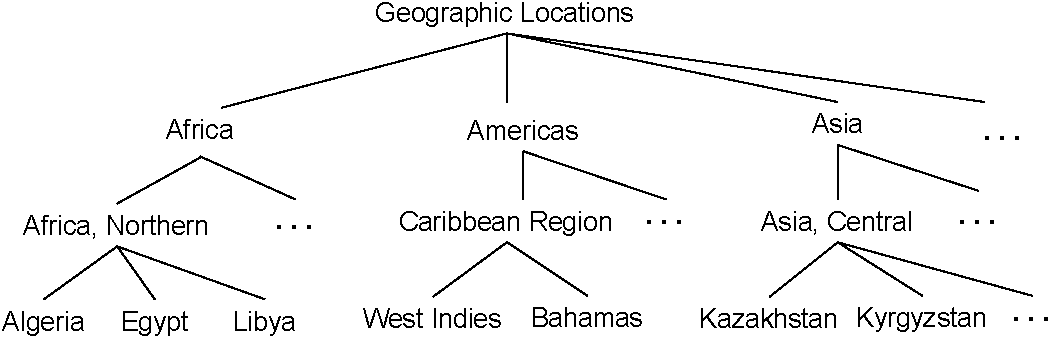
\includegraphics[width=0.45\textwidth]{figures/taxonomy}
% \caption{An example of taxonomy on ``\textsf{Geographic locations}''}
%\label{fig:taxonomy}
%\end{figure}
%
%Example extended SQL
%
%Select  T1.price, T2.price \\
%From Table T1 and T2 \\
%Where T1.area is\_a\_hypernym T2.area \\
%With taxonomy T \\
%
%
%The second SQL query:
%
%Select  T1.price, T2.price, T3.price \\
%From Table T1, T2, T3 \\
%Where T1.area is\_a\_hypernym T2.area AND T1.product is\_a\_hypernym T2.product
%


\section{Taxonomy similarity}

In this section, we show a function to quantify the similarity between two strings with taxonomy and then propose two families of efficient string join algorithms.


\subsection{Similarity functions}

Given a taxonomy tree, we borrow a labeling scheme called Dewey code, which is prefix-based scheme that records the position information of each node, according to the path from the root to the node. The IS-A relations between tree nodes whose positions are recorded in this fashion can be determined easily. For example, Figure \ref{fig:toytaxonomyexample} shows an example of taxonomy tree with Dewey codes. ``\textsf{California} (2.1.1.1)'' IS-A city in ``\textsf{U.S.} (2.1)'', since 2.1 is the prefix of 2.1.1.1.


\begin{definition}[Taxonomy Similarity]
Given two nodes $n_1$ and $n_2$ labeled with Dewey codes on a taxonomy tree, the taxonomy similarity (TS) between $n_1$ and $n_2$, TS($n_1$,$n_2$) = $\frac{|LCP(n_1,n_2)|}{max(|n_1|,|n_2|)}$, where $LCP(n_1,n_2)$  is the longest common prefix (LCP) of  $n_1$ and $n_2$.
 \end{definition}
\smallskip
\smallskip

\begin{example}
Consider Figure \ref{fig:toytaxonomyexample}, the similarity between ``\textsf{Seoul}'' (3.1.1.1) and ``\textsf{Suwon}'' (3.1.1.2) is $\frac{3}{4}$= 0.75 (as both countries are in South Korea.), and the the similarity between ``\textsf{Seoul}''  (3.1.1.1) and ``\textsf{Shenzhen}'' (3.2.1.1) is only $\frac{1}{4}$= 0.25 (as two countries are in Asia).
\end{example}


 It is easy to see that the time complexity to compute TS is $O(|n_1|+|n_2|)$ by comparing two Dewey codes sequentially.


\subsection{Join algorithms for sorted lists}

\begin{algorithm}
{\bf Input}: two sorted lists  $L_1$ and $L_2$\\
{\bf Output}: pairs $R$ =\{$(s_1,s_2) \in L_1 \times L_2$ | $TS(s_1, s_2) > \theta$\}
\begin{compactenum}[(1)]
\item {\bf FOR}  i =1 and 2 {\bf DO}
\item ~~ Initialize two pointers $C_i^1$ and $C_i^2$ to the first element of  $L_i$
\item {\bf WHILE}  $\neg$end($L_1$) and $\neg$end($L_2$) {\bf DO}
\item ~~ $min$ = $\arg\min_{i}$($cur(C_i^1)$); $max$ = $\arg\max_{i}$($cur(C_i^1)$)
\item ~~ Let $p$ denotes the prefix of $cur(C_{min}^1)$ with the length $  \lceil l \cdot \theta \rceil$
\item ~~ {\bf WHILE} (cur($C_{max}^2$) has the prefix $p$) {\bf DO}
\item ~~ ~~ ~~ {\bf IF} TS(cur($C_{max}^2$), cur($C_{min}^1$))$> \theta$ {\bf THEN}
\item ~~~   ~~ ~~ ~~ Add (cur($C_{max}^2$), cur($C_{min}^1$)) to $R$
\item ~~ ~~ ~~  advance($C_{max}^2$)
\item ~~ $C_{max}^2$ =$C_{max}^1$
\item ~~ advance($C_{min}^1$)
\end{compactenum}
\smallskip
\textbf{Function} end($L_i$)
\begin{compactenum}[(1)]
\item {\bf IF}  cur($C_i^1$) is the last element of $L_i$ {\bf THEN}
\item  ~~ RETURN TRUE
\item   {\bf ELSE} RETURN FALSE
\end{compactenum}
\caption{TS Join based on sorted labels}
\label{alg:exactjoin}
\end{algorithm}


 Given two collections of strings $S_1$ and $S_2$, assume that each string matches at most one node int a taxonomy,  then a \textit{
  similarity join} finds all pairs $(n_1, n_2) \in S_1 \times S_2$,
such that $TS(n_1,n_2)$ $>$ $\theta$, where $\theta$ is a predefined threshold. A baseline algorithm is the nested-loop join, which enumerates all string pairs to check their similarities. Its time complexity is $O(|S| \cdot |T| \cdot L)$, where $L$ is the longest string in the set. However, this baseline involves many unnecessary computation of similarity for string pairs which cannot contribute to final answers. We propose two families of optimizations to speed up the algorithm.


The first one is to sort the lists in advance. Associated with a collection $S$, there is a list $L_S$. This list contains the Dewey code of the taxonomy tree nodes that match strings in the $T$. The labels in the list are sorted by the lexicographical order. Given two sorted lists, we scan the list and output the results. The operation over lists are: \textit{advance} and \textit{end}.



Algorithm \ref{alg:exactjoin} shows the pseudo-code of a string join based on sorted lists. There are two cursors $C_1$ and $C_2$ in each list. The key idea of the algorithm is to repeatedly find the pairs pointed by $C_1$ nd $C_2$ in two lists respectively, which share the certain number of prefixes, by iterating though the list in sorted order.  In particular, Line 1-2, initialize two cursors for each list. Line 3-11 iterate two lists until two $C_1$ point to the end of their lists. For each element $e$ pointed by $C_1$, let $p$ denote the minimal prefix any answer with e has. Then Line 6-11 compare the similarity of those strings which has the prefix p and output the results.


The following lemma is a key to establish the correctness of Algorithm \ref{alg:exactjoin}.

\begin{lem} Given a string $s$ with the length $|s|$, if any string t, $TS(s,t) > \theta$,  then $s$ and $t$ share the prefix with the length of at least $|s| \cdot \theta $.
\label{lemma:sortjoinlength}
\end{lem}

\begin{theorem} Algorithm \ref{alg:exactjoin} correctly find all results for the string joins.
\end{theorem}
\begin{proof} The correctness is easy to prove, as all output pairs need the computation of similarity function in Line 7. For the completeness of the algorithm, we need to prove that there is all skipped pair are guaranteed not to contribute the final results.  In this algorithm, $C_2$ does not access every node for each $C_1$.  Lemma \ref{lemma:sortjoinlength} guarantees that each node that has the prefix p Line 5 is impossible to contribute to the final results. Therefore, the completeness is satisfied, which concludes the proof.
\end{proof}




\begin{algorithm}
{\bf Input}: two sorted lists  $L_1$ and $L_2$\\
{\bf Output}: pairs $R$ =\{$(s_1,s_2) \in L_1 \times L_2$ | $TS(s_1, s_2) > \theta$\}
\begin{compactenum}[(1)]
\item {\bf FOR}  i =1 and 2 {\bf DO}
\item ~~ Initialize two pointers $C_i^1$ and $C_i^2$ to the first element of  $L_i$
\item Let $x$ = LCP$(cur(C_1^1),cur(C_2^1))$
\item $min$ = $\arg\min_{i}$($cur(C_i^1)$); $max$ = $\arg\max_{i}$($cur(C_i^1)$)
\item {\bf WHILE}  ($\neg$end($L_1$) and $\neg$end($L_2$)) {\bf DO}
\item ~~ $z$ = $\lceil |cur(C_{min}^1)| \cdot \theta  \rceil$
\item ~~ $y = x$
\item ~~ {\bf WHILE} ($y \geq z$) {\bf DO}
\item ~~ ~~ ~~ {\bf IF} ($\frac{y}{max(|cur(C_{max}^2)|,|cur(C_{min}^1)|)}$ $> \theta$) {\bf THEN}
\item ~~ ~~ ~~ ~~ ~~ ~~ Add  the pair ($cur(C_{max}^2),cur(C_{min}^1)$) to $R$
\item ~~ ~~ ~~  advance($C_{max}^2$)
\item ~~ ~~ ~~ {\bf IF} $y > LP(C_{max}^2)$  {\bf THEN} $y$ = $LP(C_{max}^2)$
\item ~~ $C_{max}^2$ =$C_{max}^1$
\item ~~ advance($C_{min}^1$)
\item ~~  {\bf IF} $x > LP(C_{min}^1)$  {\bf THEN} $x$ = $LP(C_{min}^1)$
\item ~~ {\bf ELSE IF}  $x < LP(C_{min}^1)$  {\bf THEN}
\item ~~ ~~ ~~ ~~ Exchange the values of $min$ and $max$
\item ~~  ~~ {\bf ELSE }  $x$ = LCP$(cur(C_{1}^1),cur(C_{2}^1))$
\item ~~ ~~~~ ~~~~ ~~ $min$ = $\arg\min_{i}$($cur(C_i^1)$)
\item ~~ ~~~~ ~~~~ ~~ $max$ = $\arg\max_{i}$($cur(C_i^1)$)
\end{compactenum}
\caption{Optimized TS Join based on sorted labels}
\label{alg:LCPSortJoin}
\end{algorithm}


 Algorithm \ref{alg:exactjoin} is more efficient than the brute-force algorithm but it is not efficient to compute the LCP  because of an imbalance between effort and result in a string comparison. The computation of LCP can take a lot of time but the result is only a bit of useful information.  To speedup the query processing, we generate another index called  $LP(C_i^j)$, which is the length of the LCP between the node pointed by $C_i^j$ and its preceding node.


We now introduce an algorithm to reduce the number of string comparison in Algorithm 2. Similar to Algorithm \ref{alg:exactjoin}, we maintain two cursors C1 and C2 for each list. But the main difference between Algorithm 2 and Algorithm 1 is that we avoid the prefix checking to compute the LCP. Unlike Line 7 in Algorithm 1, Algorithm 2 do not compute LCP and compare the length of strings. We use the preprocessing LCP values and avoid the computation of LCP in most cases. Therefore, we achieve better performance.



\begin{figure}[t]
\centering
\includegraphics[width=0.25\textwidth]{figures/sortJoin}
 \caption{Illustration to the optimized sorted join algorithm. Each item is a binary tuple: (Dewey, LP).}
\label{fig:sortJoin}
\end{figure}

\begin{example} We use this example to illustrate Algorithm \ref{alg:LCPSortJoin}. The join threshold is 0.6. First the two points $C_1$ and $C_2$ point to the first elements. Then $C_2^2$ go forward to find the the first pair $(1.1.1, 1.1.3)$ to the result. Note that there is no LCP operation from 1.1.2.1 to 1.1.2.10. Then $C_1^1$ point to 1.1.2. The algorithm finds all results from 1.1.2.1 to 1.1.2.10. Their similarity is 0.75.
\end{example}

\begin{theorem} Algorithm \ref{alg:LCPSortJoin} correctly finds all results for the string joins.
\end{theorem}
\begin{proof} Algorithm \ref{alg:LCPSortJoin} follows the similar framework with Algorithm 1. But the key difference is that LCP computation is avoided. Therefore, Lemma \ref{lemma:LCPcomparison} guarantees the  correctness of the algorithm.
\end{proof}

\begin{lem} Let A, B and C be three Dewey codes,

(a) If $LCP(A,B) \neq LCP(B,C)$,  then $LCP(A,C)$ = min\{$LCP(A,B)$, $LCP(B,C)$\}.

(b) If $A>B$, $C>B$ and $|LCP(A,B)|>|LCP(B,C)|$ , then $C>B$.
\label{lemma:LCPcomparison}
\end{lem}

We can show that the worst time complexity is bounded by the product of the size of two collections plus with a sum of LCP array, which is defined as the LCP sum of alternative elements, which is better then Algorithm 1.

\begin{theorem} The TS join based on sorted lists perform the join for two tables $T_1$ and $T_2$ in $\mathcal{O}$$(S+|T_1||T_2|)$, where S= $\Sigma LCP(e,e')$, $e$ and $e'$ are two adjacent labels from the different tables in the merged sorted list.
\end{theorem}
\begin{proof}
\end{proof}

Note that the above two algorithms are not optimal, in that their computation cost is not bounded by the results size. See an example of sub-optimality as follow. Recall Figure \ref{fig:sortJoin}. If there were no element 1.1.3, then the cursors in $L_2$ move from 1.1.2.1 to 1.1.2.10 is useless. Therefore, this is not an optimal algorithm. In the next section, we seek to overcome this suboptimality using a structured: compact trie.

\subsection{Join algorithms with compact tries}

 Trie is a rooted tree with the following properties: Edges are labelled with symbols from an alphabet $\Sigma$
For every node $v$, the edges from $v$ to its children have different labels. Each node represents the string obtained by concatenating the symbols on the path from the root to that node. The space requirement can be problematic, since typically each node needs
much more space than a single symbol.

Compact tries reduce the number of nodes by replacing branchless path segments with a single edge.
We can enhance the compact trie by adding the integer to indicate the shortest real element under the subtree.

%\begin{figure}[t]
%\centering
%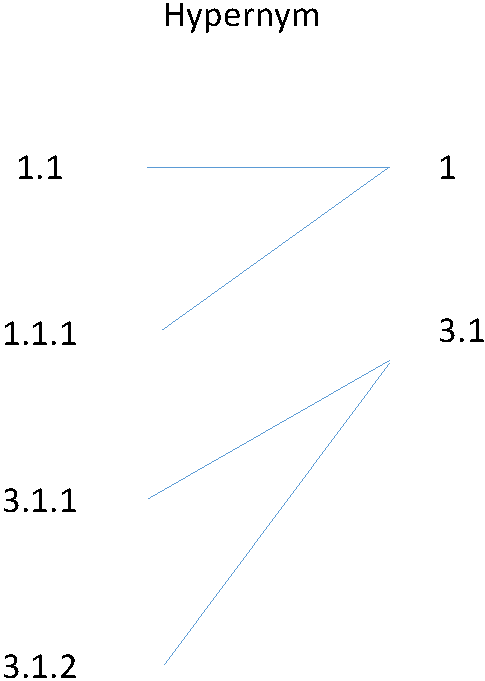
\includegraphics[scale=0.4]{figures/labeljoins}
% \caption{Join inverted lists}
%\label{fig:invertedlist}
%\end{figure}

The worst case complexity is $O(N^2)$, because the algorithm may compute each pair of strings with the prefix $p$. But this algorithm will skip many pairs of string for comparison. A theoretical analysis based on a random string model show that the average complexity is $O(\frac{N^2}{S^{\lfloor (1-\theta) \cdot l \rfloor}})$, where $N$ is the total number of elements in each list and $S$ is the maximal width of the taxonomy.




\begin{figure}[t]
\centering
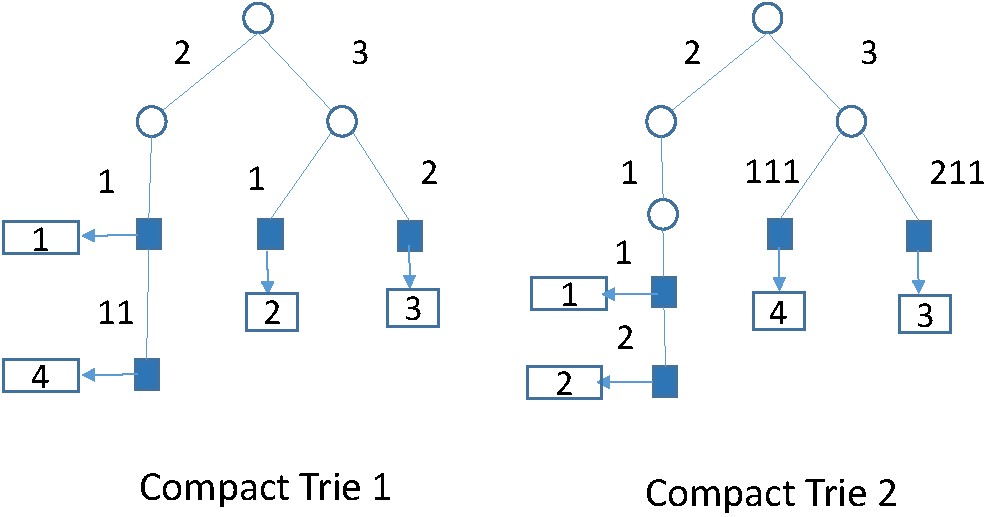
\includegraphics[width=0.35\textwidth]{figures/prefixTrees}
 \caption{An example of TS join based on prefix trees (a circle means an internal element, but a rectangle means a real element)}
\label{fig:taxonomyexample}
\end{figure}



\begin{algorithm}
{\bf Input}: two collections of taxonomy nodes $S_1$ and $S_2$,  a threshold $\theta$ \\
{\bf Output}: string pairs $(s_1,s_2) \in S_1 \times S_2$, s.t. $TS(s_1, s_2) > \theta$
\begin{compactenum}[(1)]
\item Let $T_s$ and $T_t$ denote two compact tries for $S$ and $T$ respectively. 
\item Initialize two cursors in two tries.
\item {\bf WHILE} $\neg end(T_s) \wedge  \neg end(T_t)$ {\bf DO}
\item  ~~ $min$ = $\arg\min_{i}$($cur(C_i^1)$); $max$ = $\arg\max_{i}$($cur(C_i^1)$)
\item  ~~ {\bf IF} (possibleMatch(cur($T_{min}$),cur($T_{max}$))) {\bf THEN}
\item ~~ ~~ {\bf  IF} ($T_{min}$ is a real element)   {\bf THEN} Find(cur($T_{min})$,cur($T_{max}$))
 \item ~~~~ advance($T_{min}$)
 \item ~~ {\bf ELSE} Jump($T_{min}$)
 \item ~~ advance($T_{min}$)
\end{compactenum}
\smallskip
\textbf{Function} possibleMatch($s_1$,$s_2$)
\begin{compactenum}[(1)]
\item  $x = LCP(s_1,s_2)$
\item {\bf IF}  $(x > \theta \cdot min (s_1, s_2 )$  {\bf THEN} RETURN TRUE
\item   ~~ {\bf ELSE} FALSE
\end{compactenum}
\smallskip
\textbf{Procedure} Jump($T$)
\begin{compactenum}[(1)]
\item  read the next element that is not a descendant with the depth-first traversal
\end{compactenum}
\smallskip
\textbf{Procedure} Find($s_1$,$s_2$)
\begin{compactenum}[(1)]
\item  $x = LCP(s_1,s_2) $
\item {\bf IF} ( $|s_2| < max(\frac{x}{\theta},|s|)$) {\bf THEN}
\item ~~~~ {\bf FOR EACH} $i$=$|s_2|$ to $ \lceil max(\frac{x}{\theta},|s|) \rceil -1 $ {\bf DO}
\item ~~~~~~~ Add all real nodes under $s_2$ with the length $i$ to R;
\end{compactenum}
\caption{String joins with compact tries}
\label{alg:compactTrieJoin}
\end{algorithm}

\begin{theorem} Given two collections of nodes and a threshold $theta$, Algorithm \ref{alg:generaljoin} correctly finds all pair $n_1$ and $n_2$ such that $TS(n_1,n_2) > \theta$.
\end{theorem}


\begin{lem} Given two labels $s$ and $t$,  assume that $LCP(s,t) = x$. without the loss of generality, assume that $s<t$ by the lexicographical order, $TS(s,t) > \theta$ if and only if  $ x > \theta |s| $ and $  |t| < max(\frac{x}{\theta},|s|)$.
\end{lem}
\begin{proof}  $TS(s,t) > \theta$ $\Leftrightarrow$ $\frac{x}{|s|+|t|-x} > \theta \Leftrightarrow |t| < (\frac{1}{\theta}+1)x-|s|$. In addition, note that $|t| \geq x$. Then $x < (\frac{1}{\theta}+1)x-|s|$ $\Rightarrow$ $x > \theta |s| $, which concludes the proof.
\end{proof}


\smallskip
\smallskip

\begin{example}
Consider the example in Figure \ref{fig:taxonomyexample}, $\theta$=0.4. First, the cursors point to 2 and 2. possibleMatch return true. But 2 is not the real elements.  Then advance. Now $s_1$ =2.1 in $T_1$  and $s_2$=2.1.1 in $T_2$. Both real nodes. $x$=2.1, ($\frac{1}{\theta}+1)|x|-|s_1|$ = $5 > 3$. Therefore, (2.1, 2.1.1) and (2.1, 2.1.1.2) are added to the result pairs. Then the cursor advances, when $s_1$ =2.1.1.1, the result pair (2.1.1.1, 2.1.1.2) are added. Subsequently, the other two pairs (3.1, 3.1.1.1) and (3.2, 3.2.1.1) are added.
\end{example}

\smallskip
\smallskip

We next show the optimality: Given two compact tries, Algorithm \ref{alg:generaljoin} takes each node and find the  matching node with the trie operations. Therefore, each accessed pair $C_1$ and $C_2$ belong to the final results. Since the operation of output Line is equal to the size of the final results: we have the following optimality result:

\begin{theorem}   The computing cost of Algorithm \ref{alg:generaljoin} is linear to the sum of the size of the input and output.
\end{theorem}







\section{String similarity joins with taxonomy}


In this section, we discuss how to use taxonomy on string similarity joins. For this purpose, we first extend the Jaccard similarity to utilize the taxonomy. Then we propose several algorithms and optimizations for the problem of similarity joins with taxonomy.



\subsection{Similarity measures}


We define the taxonomy similarity between two strings:

\begin{definition}[Taxonomy intersection]
Given two token sets $S_1$ and $S_2$, and a taxonomy $\mathcal{T}$, we say an element (token) $e \in S_1 \bigcap_T S_2$, if $ \exists E \subseteq S_1$ and $e \in E$, and $\exists T \subseteq S_2$, s.t. $\exists (E,T) \in \mathcal{T}$.\end{definition}


\noindent \textbf{Remark.}  Given two strings $s$ and $t$, it is clear that $|s \cap t| \leq min (|s|,|t|)$. But based on the taxonomy intersection, it is possible that $|s \cap_T t| > |s| $ or $|s \cap t| > |t| $. For example, s=``California'', t=``U.S.'', $|s \cap_T t|$ = 2. But it is still true that $|s \cap_T t| < |s \cup t|$

We need to define a new similarity:

Given a token set S which include two parts: $S_1$ and $S_2$, where $S_1$ contains only unique token and $S_2$ is the taxonomy token. Then the similarity between S and T is defined as

$\frac{min(|S_2|,|T_s|)}{|S_1|+|T_1|+min(|S_2|,|T_s|)}$

\begin{definition}[Taxonomy-based Jaccard]   Given two sets of tokens $S_1$ and $S_2$,  the taxonomy-based Jaccard (TJ) between $S_1$ and $S_2$ is that:

\begin{equation}
TJ(S_1,S_2)=  \frac{(S_1 \bigcap_T S_2) \bigcup (S_1 \bigcap S_2) }{S_1 \bigcup S_2}
\end{equation} \end{definition}

\begin{algorithm}
{\bf Input}: two strings $s_1$ and $s_2$, a taxonomy $\mathcal{T}$ \\
{\bf Output}: $TJ(s_1,s_2,\mathcal{T})$
\begin{compactenum}[(1)]
\item Let $S_T $ to contain all tokens for taxonomy-based intersection. Initially, $S_T = \emptyset$.
\item Let $L_1$ (resp. $L_2$) denote the applicable taxonomy node list for $s_1$ (resp. $s_2$);
\item Scan $L_1$ and $L_2$ sequentially to find any matching pair $n_1 \in L_1$, $n_2 \in L_2$, s.t. ($n_1$,$n_2$) has the IS-A relation in $\mathcal{T}$;
\item Add all tokens $t \in n_1 \cup n_2$ to the set $S_T$;
\item  return $\frac{S_T \cup (|s_1 \cap s_2|)}{|s_1 \cup s_2|}$;
\end{compactenum}
\caption{String joins with taxonomy}
\label{alg:exactjoin}
\end{algorithm}

The time complexity of the TJ is $O(|s_1|+|s_2|+|n_1|+|n_2|)$, where $n_1$ (resp. $n_2$) denotes all applicable taxonomy nodes for string $s_1$  (resp. $n_2$). Assume that the preprocessing step finds the taxonomy relation for each string. Then the online algorithm only needs to find the matching IS-A relation between two strings to compute the intersection set with taxonomy.

\subsection{String similarity join algorithms}


%\begin{figure}[t]
%\centering
%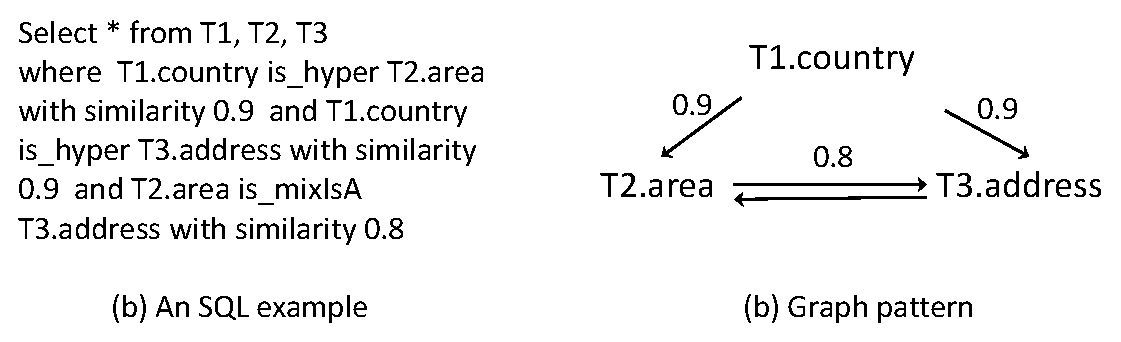
\includegraphics[scale=0.4]{figures/tgsql2}
% \caption{Taxonomy graph example }
%\label{fig:similaritygeaph}
%\end{figure}

We would formulate the string similarity join problem and develop the corresponding algorithms. Given two collections of strings $S$ and $T$, a taxonomy tree
$\mathcal{T}$, and a similarity threshold $\theta$, a \textit{string
  similarity join} finds all string pairs $(s, t) \in S \times T$,
such that $JT(s,t,\mathcal{T})$ $>$ $\theta$, where \textit{JT} is
 the Jaccard-taxonomy similarity functions defined above. Two join algorithms would be proposed in the following subsections.



\textbf{Baseline algorithm}. We can use the similar algorithm as that in string exact join with taxonomy. And then use these candidate for filtering. But this baseline algorithm has one limitation that there are too many candidates. Then we show how to perform the second filtering to reduce the number of candidate pairs.

\textbf{Signature-based index}. Given a string s with length $|s|$, then the size of signature is $\lceil (1-\theta)|s| \rceil$. But if the signatures involve the taxonomy, then we cannot make this argument.

But if in some real cases, we select the word from taxonomy as signatures. Therefore we need to compute a relax maximum similarity. In this case, we still do not need to retrieve the whole string to compute real similarity.

Given as string $s$, assume that its applied taxonomy node is $n$.

In this paper, we propose a new index which combine a signature filters and a length together with a bit-matrix, which extends bloom filter to two dimensions.

In the literature, the current "modus operandi" is called \textit{prefix filter}, which is based on the intuition that if two canonicalized records are similar, some fragments of them should overlap with each other, as otherwise the two records
won't have enough overlap. This intuition can be formally captured by the prefix-filtering
principle \cite{conf/icde/ChaudhuriGK06} rephrased below.

\begin{lem} (\textsc{Prefix filter principle}) \cite{conf/icde/ChaudhuriGK06} Given an
ordering $O$ of the token universe $U$ and two strings $s$ and $t$, each with tokens sorted in the
order of $O$.   If Jaccard($s, t$) $> \theta$, then the first $\lceil(1-\theta)|s|\rceil$ smallest
tokens of $s$ and the first $\lceil(1-\theta)|t|\rceil$ smallest
tokens of $t$  must share at least one token.
\end{lem}

\subsubsection{N-ary prefix scheme}




Given a string $s$, we can construct the $n$-ary prefix token combination as follows:  Given an
ordering $O$ of the token universe $U$, we select $n$ tokens from the first $\lceil (1-
\theta) \cdot |s| \rceil + n -1$ in $s$. Then let $B^s_n$ denote the set to contain all $n$-combinations. That is  $|B^s_n|$= $\binom{(1-\theta)|s|+n-1}{n}$.

\begin{lem} (\textsc{N-ary signature principle}) Given two strings $s$ and $t$ and their n-ary signatures $T^s$ and $T^t$ respectively, if Jaccard($s, t$) $> \theta$, then $T^s \cap T^t \neq \emptyset$.
\end{lem}

Given a string s=\{A,B,C,D,E\}. If we use the prefix filtering, then the signature is A and B. Assume that $\theta$=0.75, (1-0.75)*5=1.25 and $\lceil 1.25 \rceil$=2. But in our bi-tuple scheme, we select two tokens as the signatures, including \{A,B\},\{A,C\},\{B,C\}.

Similarly, we can develop a 3-tuple signature. we select three tokens as the signatures, including $\binom{4}{3}$=4, i.e. \{A,B,C\}, \{A,C,D\}, \{B,C,D\}, \{A,B,D\}.

Furthermore, we can extend to 4-tuple signature, that is $\binom{5}{4}$=4, i.e. \{A,B,C,D\}, \{A,C,D,E\}, \{A,B,D,E\}, \{A,C,D,E\}, \{B,C,D,E\}.

One question is how to select the number $n$ for n-tuple scheme. What is the optimal value of $n$? Let $t= (1-\theta)|s|$, that is, $O((t+n-1)^{n})$. If n is too large, then there are many signatures, it may not be an optimal solution. Therefore, the key point is how to decide a good $n$?


\subsubsection{N-ary prefix scheme with taxonomy}

 Given a string s=\{A,B,C,D,E\}, assume that we use 3-tuple signature, $\binom{4}{3}$=4, i.e. \{A,B,C\}, \{A,C,D\}, \{B,C,D\}, \{A,B,D\}.

For each tokens, there are two cases, that is, it contains a taxonomy word, say $t \in w$. Then we use $w$ to replace $t$. Note that $t$ may belong to multiple taxonomy words. Therefore, ($w_1, w_2, \cdots, w_3$)

Continue the above example, assume that $DE$ = 1.1. Note that $E \in s $, but $E$ does not belong to the signatures. Then the new three signatures:  \{A,C,1.1\}, \{B,C,1.1\}, \{A,B,1.1\}.

\noindent \textbf{Composite signatures} Given a string $s$, a composite signature of $s$, denoted by C-Sig($s$) includes two types of elements $T$ and $N$, where $T$ is a set of tokens and $N$ is a set of T-nodes.

Given an
ordering $O = (U_1 , U_2 )$ of the token universe $U_1$ and $U_2$, where $U_1$ denotes the set of non-taxonomy tokens and $U_2$ is the set of taxonomy tokens. Let $P_s$ denote the smallest $\lceil(1-\theta)|s|\rceil$ tokens.

%\begin{lem} (\textsc{Prefix filter principle with taxonomy})  Given two strings $s$ and $t$ with n-ary prefix signatures, if TJ($s, t$) $\geq \theta$, then one of the following cases holds:
%
% \begin{itemize}
%   \item $P_s \cap P_t \neq \emptyset$, or
%   \item  $T_s \cap A_t \neq \emptyset$ or $T_t \cap A_s \neq \emptyset$
% \end{itemize}
%
%\end{lem}
%


%\begin{lem} (\textsc{Prefix filter principle with taxonomy})  Given two strings $s$ and $t$ with n-ary prefix signatures, if TJ($s, t$) $\geq \theta$, then one of the following cases holds:
%
% \begin{itemize}
%   \item $P_s \cap P_t \neq \emptyset$, or both of the conditions satisfy:
%   \item  $\exists sig^s \in P_s, sig = sig^s_{token} \cup sig^s_{tax} s.t. \exists sig^t \supseteq sig^s$ and $sig^s_{tax} \subseteq Tax(t)$ and
%    \item  $\exists sig^t \in P_t, sig = sig^t_{token} \cup sig^t_{tax} s.t. \exists sig^s \supseteq sig^t$ and $sig^t_{tax} \subseteq Tax(s)$
% \end{itemize}
%
%\end{lem}

A signature set $P$ for a string $s$ is a binary tuple ($T,N$), where $T$ is a set of tokens and $N$ is a set of taxonomy nodes.

\begin{definition} [Signatures match strings]
Given a signature set $P = (T,N)$ and a string $s$, we say $P$ matches $s$, denoted by $P \vdash s$ if $N \subseteq N^s$, where $N^s$ is a set of applicable taxonomy nodes of $s$ and  there exits a signature set $P' = (T',N')$ of $s$, s.t. $T \subseteq T'$.
\end{definition}


\begin{lem} (\textsc{Composite signatures principle})  Given two strings $s$ and $t$ with signatures $P^s$ and $P^t$ respectively, if TJ($s, t$) $> \theta$, then $P^s \vdash t$ and $P^t \vdash s$.

\end{lem}

For example, consider two strings s=\{A,B,C,D,E\} and t=\{F,G\}. Assume that $t_1$ = (ACD,G) is an IS-A relation and the $|s \cap_T t| $=4, $JT(s,t)$ = $\frac{4}{7}$= 0.57.
If the threshold $\theta =$ 0.5, then  $\lceil (1-\theta) \times 5 \rceil$= 3 for $s$ and $\lceil (1-\theta) \times 2 \rceil$= 1. Assume that the order of non-taxonomy tokens $O_1$= \{$B, E, F$\} and the order of taxonomy tokens is $O_2$ = \{$A, C, D, G$\}. So the signature of $s$ is \{B,E,A\}, and an IS-A relation $T_s$ = (ACD,G). The signature of $t$ is \{F\} and $A_t$ = (ACD,G). $ T_s \cap A_t \neq \emptyset$.

\subsubsection{Similarity join algorithm}

We discuss the similarity join algorithm based on the above n-ary composite signature filters.


\begin{algorithm}
{\bf Input}:  two collections of strings $S$ and $T$ and the threshold $\theta$ \\
{\bf Output}: result pairs ($s,t$)$\in S \times T$, s.t. JT($s,t$)$> \theta$
\begin{compactenum}[(1)]
\item Find candidate pairs $C_1$ = \{$(s,t) |$  $P^s \vdash t$\};
\item Find candidate pairs $C_2$ = \{$(s,t) |$  $P^t \vdash s$\};
\item  $C= C_1 \cap C_2$;
\item FOR EACH ($s,t$)$\in C$
\item RETURN all pairs s.t. $JT(s,t) > \theta$
\end{compactenum}
\caption{String joins with taxonomy}
\label{alg:exactjoin}
\end{algorithm}

For each table, we can generate four inverted lists for strings: (1) a list $L_I$ for tokens where the signatures of strings contain only tokens; (2) a list $L_{II}$ for taxonomy nodes where the signatures of strings contain only nodes; (3) a list $L_{III}$ for tokens where the signatures of strings contain both tokens and nodes; (4)  a list $L_{IV}$ for nodes where the signatures of strings contain both tokens and nodes.


\begin{algorithm}
{\bf Input}: two collection of strings $S$ and $T$ and their corresponding inverted lists $L_I^S$,  $L_{II}^S$, $L_{III}^S$, $L_{IV}^S$, $L_N^T$ \\
{\bf Output}: string candidate pairs \{$(s,t) |$  $P^s \vdash t$, $s \in S$ and $t \in T$\}
\begin{compactenum}[(1)]
\item  $C_1$=$\displaystyle\bigcup_{g \in L_I^S \cap L_I^t} (L_I^s(g) \times L_I^t(g)) $;
\item  $C_2$=$\displaystyle\bigcup_{n \in L_{II}^S \cap L_N^t} (L_{II}^s(n) \times L_N^t(n)) $;
\item  $C_3$=$\displaystyle\bigcup_{g \in L_{III}^S \cap L_{III}^t} (L_{III}^s(g) \times L_{III}^t(g)) $;
\item  $C_4$=$\displaystyle\bigcup_{n \in L_{IV}^S \cap L_N^t} (L_{IV}^s(n) \times L_N^t(n)) $;
\item   Return $C_1 \cup C_2 \cup (C_3 \cap C_4)$;

\end{compactenum}
\caption{String candidate pairs}
\label{alg:exactjoin}
\end{algorithm}

\begin{table*}[t]
\centering
\begin{tabular}{|@{\hspace{1mm}}c@{\hspace{1mm}}|@{\hspace{1mm}}c@{\hspace{1mm}}|}
%{|p{1cm}|p{1cm}|p{1cm}|p{1cm}|p{1cm}|p{1cm}|p{1cm}|}
%|c|m{6cm}|
\hline
 \textbf{Symbols} & \textbf{Definitions}  \\
  \hline \hline

  $L_I(g)$ &    $\forall s \in L_I(g)$,  s.t. $\exists  R  \in C$-$Sig(s)$, $R$ contains only tokens and $g \in R$ \\

   $L_{II}(n)$ & $\forall$ $s \in L_{II}(n)$, s.t. $\exists  R  \in C$-$Sig(s)$, $R$ contains only T-nodes and $n \in R$    \\

   $L_{III}(g)$ & $\forall$ $s \in L_{III}(g)$, s.t.  $\exists R  \in C$-$Sig(s)$, $R$ contains both tokens and T-nodes, $g \in R$    \\

  $L_{IV}(n)$ &  $\forall s \in L_{IV}(n)$, s.t. $\exists R  \in C$-$Sig(s)$, $R$ contains tokens and T-nodes and $n \in R$    \\

$L_{N}(n)$ &  $\forall s \in L_{N}(n)$, s.t. $n$ is an applicable T-node of $s$   \\

  \hline
\end{tabular}
\caption{Summary of definitions of various inverted lists}
\label{tab:symbols}
\end{table*}


\begin{table*}[t]
\centering
\begin{tabular}{|@{\hspace{1mm}}c@{\hspace{1mm}}|@{\hspace{1mm}}c@{\hspace{1mm}}|@{\hspace{1mm}}c@{\hspace{1mm}}|@{\hspace{1mm}}c@{\hspace{1mm}}|}
%{|p{1cm}|p{1cm}|p{1cm}|p{1cm}|p{1cm}|p{1cm}|p{1cm}|}
%|c|m{6cm}|
\hline
 \textbf{ID} & \textbf{Strings} &  \textbf{Signatures} &    \textbf{C-Sig} \\
  \hline \hline

  $q_1$ & Suwon and Seoul in South Korean  &  (Suwon, and), (Suwon Seoul), (and, Seoul)  & () \\

   $q_2$ & Seoul, South Korean in Asia  & (Seoul, South), (Seoul, Korean), (Seoul, Korean) &   3.1.1.1, in \\

   $q_3$ &  two states: California and Michigan, U.S. &  (two, states), (two, California), (states, California) & (two, states), (two, 2.1.1), (states, 2.1.1)  \\
   $q_4$ & two cities: Detroit and Los angles & (two, cities), (two, Detroit), (cities, Detroit) &  (two, cities), (two, 2.1.2.1), (cities, 2.1.2.1) \\


  \hline
\end{tabular}
\caption{An example to illustrate the string similarity join algorithm}
\label{tab:example}
\end{table*}


\begin{example} We use Table as an example to illustrate the algorithm.

\end{example}

\subsubsection{Comparison with other schemes}


\begin{table}[t]
\centering
\begin{tabular}{|@{\hspace{1mm}}c@{\hspace{1mm}}|@{\hspace{1mm}}c@{\hspace{1mm}}|@{\hspace{1mm}}c@{\hspace{1mm}}|}
%{|p{1cm}|p{1cm}|p{1cm}|p{1cm}|p{1cm}|p{1cm}|p{1cm}|}
%|c|m{6cm}|
\hline
 \textbf{Methods@{}} & \textbf{Signature size} &  \textbf{Filtering power} \\
  \hline \hline

  Prefix & (1 -$\theta$)$|s|$ & Optimal \\


   PartEnum & CPU:  O($1.2002^{|V|} \cdot |V|^{O(1)}$ ) & Optimal \\

   LSH & CPU:  O($|V|$log$|V|$+$|E|$)  & $(2\bar{d}+3)/5$  \\

   Composite Prefix & I/O: O(sort($|E|$+$|V|$))   & No bound \\


  \hline
\end{tabular}
\caption{Time and  I/O cost and performance}
\label{tab:complexity}
\end{table}

 We compare our composite prefix filter with state-of-the-art filters. The objective of the filters is to prune dissimilar strings as many as possible. They require to select a set of q-grams from each of two strings as signatures, denoted as Sig(r) and Sig(s), and compare the two q-gram sets to check whether they share common signatures. Pruning power and filtering cost are two important issues in designing filters.

We first consider the pruning power. One one hand, the smaller the production size of the two signature sets $|Sig(r)| \times$
$|Sig(s)|$, the smaller probability they share common q-grams, and thus the higher pruning power. On the other hand, the number of matching q-grams cannot exceed the smaller signature size of the two strings, min($|Sig(r)|, |Sig(s)|$). Thus
we can use the production size of two signature sets and
the smaller signature set size to evaluate the pruning power. We then evaluate the filtering cost. As the q-gram sets
are sorted, we can use a merge-join algorithm to find the
matching q-grams if there is no index, the filtering cost depends on the sum of signature set sizes of the two strings,
$|Sig(r)|$ + $|Sig(s)|$. Table 3 compares the pruning power and filtering cost of state-of-the-art q-gram-based filters used in AllPair, ED-Join, Qchunk-IndexChunk and Qchunk-IndexGram.

\smallskip

\noindent \textbf{Length filters}


\subsubsection{Composite signature: Performance}

In this section, we cover various aspects of Composite-signature scheme's performance.
We begin by proving that it has good asymptotic performance: For a particular setting of n1 and n2, we can prove
that it provides good filtering effectiveness (i.e., generates only a few false positive candidate pairs) with few signatures per input set.

\begin{theorem} If the Jaccard similarity of two strings are greater than $\theta$, then $Sig(u) \bigcap Sig(v) = \varnothing$ with probability 1-o(1). For this setting of parameters, the number of signature per string is O().
\end{theorem}


Given a $n$-tuple composite filter, we estimate its filtering effectiveness.

We assume that there are $N$ tokens in all tables and the length of each string is $s$.

The possibility of false positive for a string pair $s, t$ is that $P(E_A | E_B)$, $E_B$ means that  $sim(s,t) < \theta$; $E_A$ means that $s$ and $t$ pair cannot be pruned away with the filter.

First consider the 1 prefix signature. We computer $P(E_A, E_B)$, that is, the prefix signature cannot prune away the pair of $Jaccard(s,t) < \theta$

Let $\lambda$ = $(1-\theta)s$ signatures for $t$.

Since $|s| = |t|$ and   $Jaccard(s,t) < \theta$ $\Longleftarrow$ $ |s \cap t| < |s| \cdot \theta$.

%\subsection{Count-Min estimation}
%
%In order to quickly decide if the number of pairs after composite filters, we develop a count-min estimation to quickly determine which $n$ is good for filtering. See the following two examples for joins.
%
%See the example in Figure \ref{fig:signature_example1}. In this example, $\theta$ = 0.8. If we use the 1-element signature, then we cannot prune away any string pair. In signature 2, we use 2-element signature, then there is no candidate. Therefore, the filtering power is better.
%
%Further, when we consider the taxonomy ABCD ISA AGK, shown in Figure \ref{fig:signature_example1}. Then there is one answer pair (s1,t1). The new signature include the taxonomy ID 1.1 and 1  as shown.
%
%\begin{figure}[h]
%\centering
%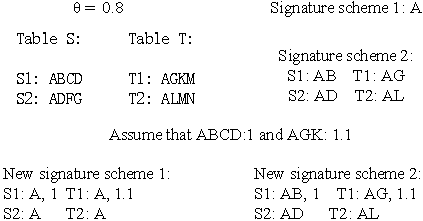
\includegraphics[scale=0.8]{figures/signature_example1}
% \caption{Illustration to the difference of signature schemes}
%\label{fig:signature_example1}
%\end{figure}
%
%A Count-Min (CM) sketch with parameters ( $\varepsilon, \delta$) is represented by a two-dimensional
%array counts with width $w$ and depth $d$. Given parameters ($\varepsilon, \delta$), set
%$w$ = $\lceil \frac{e}{\varepsilon} \rceil$ and $d$ = $\lceil ln \frac{1}{\delta} \rceil $. Each entry of the array is initially zero.
%
%
%When a data item ($w,i$) arrives, meaning that the signature $w$ has the length $i$, then $i$ is added to one cell in each row; the counter is determined by $h_j$. Formally, set $\forall 1 \leq j \leq d$, then count[j,$h_j(i)$]
%
%
%The space used by Count-Min sketches is the array of $wd$ counts, which takes $wd$ words, and $d$ hash
%functions, each of which can be stored using 2 words when using the pairwise functions described in [27].
%
%Estimation procedure. Our estimation for $S \bigodot T $ = $min_j S_j \bigodot T_j $
%
%
%\begin{theorem}
%With a probability 1- $\delta$, The upper bound and lower bound of Composite signature estimation is
% $S \bigodot T $ and  $S \bigodot T $ + $\varepsilon |S| |T|$, respectively.
%\end{theorem}
%
%\begin{theorem}
%Our composite signature estimation estimates the lower and upper bounds of algorithms by keeping space $O(\frac{1}{\varepsilon} \log \frac{1}{\delta})$ and
%\end{theorem}
%
%\subsubsection{Estimation with length filters}
%
%When we use the CountMin sketch to estimate the effectiveness of length filter. It is to



\subsection{Extensions for flexible query thresholds} \label{subsec:flexible}

In the previous sections, our model assumes that the search threshold is fixed, and only the query can be changed online. However, in practice users might change the threshold at query-time. Therefore, we now move to a more general case, where both the search string and the threshold are flexible at query-time. The new challenge here is that we do not know the threshold in advance and thus we cannot determine the number of signatures of each record. A na\"{i}ve method is to compute the signatures of records in the table online according to the given threshold, which  is clearly prohibitively expensive. Next we build a new index called \textit{FSI-trees} (Flexible Signature Indexing) by extending SI-trees to solve this problem.

Suppose that all meaningful thresholds distribute in the range between 0.99 to 0.50. Then we select some \textit{representative thresholds}, e.g. 0.95, 0.90, etc.   For each representative threshold, we generate signatures for each record. See an example in Figure \ref{fig:FSI}(a). Note that the signatures of a string for lower thresholds are guaranteed to become signatures of that for higher thresholds. To build an FSI-tree,  the length and fence entries of SI-trees remain the same. But each fence entry points to a set of I-lists which come from \textit{all} representative thresholds. Further, each element in the I-list of a signature token $s$ is a binary tuple ($q$, $\theta$), where $q$ is a record ID and $\theta$ is the minimal threshold for which this signature $s$ appears in $q$. For example, in Figure \ref{fig:FSI}(b), the token ``\textsf{Computing}''  is a signature of $q_1$ for all thresholds $\geq 0.5$.

We extend the QP-search algorithm for flexible thresholds. The algorithm almost remains the same, but  the only  change (See Algorithm \ref{algo:QP-flexible}) is that we select the string candidates in I-lists by checking their thresholds (Line 3).

An astute reader may notice that our method possibly introduces more candidates because of the gap between representative thresholds and online thresholds. For example, given a query threshold 0.83, suppose that the closest representative threshold is 0.80. Then  the number of signatures for threshold 0.80  may be greater than that for 0.83. But we argue that the problem  has actually a little impact on the final performance of query processing. To understand this, assume that gap between two representative thresholds is no more than 0.05 (that means, only 11 representative thresholds are ``materialized'' with signatures between 0.99 and 0.50). It can be proved that given a string $s$, the difference between the numbers of signatures for thresholds $\theta_1$ and $\theta_2$ is $\lceil  |\theta_1 - \theta_2|   \cdot |s| \rceil$. Considering a string $|s|$=10, we have 0.05 * 10 =0.5, That is, for most records in the table, the extra number of signatures due to the thresholds gap  is bounded by 0.5. Therefore, as our experimental results show in Section \ref{subsec:searchalgorithms}, the performance of our algorithms for flexible thresholds is comparable to that for static thresholds.





\input{updatingTaxonomy}

\input{extension}

\section{Experimental analysis}

In this section, we evaluate the experimental results of
the proposed exact-join and approximate-join algorithms.

 We will compare
their effectiveness on the following datasets from different
application scenarios in Java $1.6.0$ and run on a
Windows XP with dual-core Intel Xeon CPU 4.0GHz, 2GB RAM, and a 320GB hard disk.


\subsection{Datasets}

One possible dataset is about the model of CPU:
%http://archive.ics.uci.edu/ml/machine-learning-databases/cpu-performance/

%http://arthropods.eugenes.org/lucegene_arthropod/search

%http://arthropods.eugenes.org/lucegene_arthropod/resultxsl.jsp




To evaluate the impact of taxonomy information on classification performance, we generated taxonomies over each dataset.
While aggregation trees on continuous attributes have been generated by applying discretization procedures, aggregation trees
on nominal attributes are analyst-provided. Note that, in real-life contexts, aggregation trees may be semi-automatically derived, for instance, from lexical or geographical databases (e.g., the WordNet Lexical Database [18]). A more detailed description of the
applied multiple-taxonomies follows.

As a subject matter taxonomy for our expert matching
in this medicine domain, we used the Medical Subject Head-
ings (MeSH)\footnote{https://www.nlm.nih.gov/mesh} that is a biomedical controlled vocabulary
consisting of 26k+ biomedical terms arranged in a taxonomic
structure introduced by National Library of Medicine
(NLM). The benefits of using MeSH terms have been increasingly
highlighted in various applications for biomedical
concept and knowledge extraction from text [11].


We use three datasets: Consensus data (\textbf{Consensus}),
Academic data  (\textbf{Academy}), and Life science data
(\textbf{Life}). These datasets differ from each other in terms of rule-number, rule-complexity, data-size and string-length. Our goal in choosing these diverse sources is to understand the usefulness of algorithms in different real world environments.

\smallskip
\noindent \textbf{{Consensus data}}: Extraction was done by Barry Becker from the 1994 Census database. native-country: Include 32561 instances, we can perform the similarity joins on multiple column, including countries, occupation, marital-status, education and workclass. The feature of this dataset is to perform the similarity join against multiple columns.

\noindent \textbf{{Academic data}}: We collected 10,000 affiliations of authors for computer science.
We build a taxonomy tree which include the country and city and the university names.


\noindent \textbf{{Life science data}}: Designing data integration solutions in the context of the Life Sciences
must take into account the specific properties of the domain [3,
4]. These are related to (i) the way biological data is produced
and stored within biological databases (BDB), (ii) the fact that
biology is a science in constant evolution, and (iii) the fact
that BDB users are from various communities.
Regarding the first point, primary BDB store data that is
close to the raw experimental result (e.g., DNA sequences),
while secondary BDB manage information obtained after
various steps of analysis and careful curation, grouped around
increasingly complex entities (e.g., genes, diseases, pathways
etc.). While (discrete, string-type) sequences were the main
kind of raw data to integrate 20 years ago, today various �C
omics data set (transcriptomics, proteomics,etc.), often
consisting of quantitative measurements, are of equal
importance. Secondary BDBs heavily import data from other
BDB and are mostly maintained by human curators; they may
be complementary but also could be redundant and divergent
(especially when experts disagree). Because humans offer
unrivaled precision, manual curation still predominates,
despite its high cost and obvious problems of scalability.
The number of BDB is increasing steeply; currently more
than 1,200 BDBs are publicly available. This led to the call
for DI systems with extreme scalability in the number of
sources. However, in reality the usage of these databases is
Zipf-distributed [2], and there are only a few projects that
work with more than, say, 20 different data sources.
We obtained one million gene/protein records
from the Expasy website ({\footnotesize http://www.expasy.ch/sprot}).
Each record contains an identifier (ID) and its name.
%For example, the two records, \textit{(O00203, Adapter-related protein complex 3
%beta-1 subunit)} and \textit{(O00203, AP-3 complex subunit
%beta-1)}, refer to the same gene as they have the same ID.
In this dataset, each ID has $5\sim22$ synonyms. We generated 10,000 synonym rules describing gene/protein
equivalent expressions.


\begin{table}[t]
\centering
\begin{tabular}{|@{\hspace{1mm}}c@{\hspace{1mm}}|@{\hspace{1mm}}c@{\hspace{1mm}}|@{\hspace{1mm}}c@{\hspace{1mm}}|@{\hspace{1mm}}c@{\hspace{1mm}}|}
%{|p{1cm}|p{1cm}|p{1cm}|p{1cm}|p{1cm}|p{1cm}|p{1cm}|}
%|c|m{6cm}|
\hline
 \textbf{Dataset} & \textbf{\# of strings} &  \textbf{string length} & \textbf{Taxonomy size} \\
  \hline \hline

  Consensus & 10,000 & 5 & 2,000 \\

   Academy & 10,000 & 5 &  2,000 \\

   Life & 10,000  & 5 & 2,000  \\

  \hline
\end{tabular}
\caption{Time and  I/O cost and performance}
\label{tab:data}
\end{table}


\begin{figure}
  \small
  \centering
  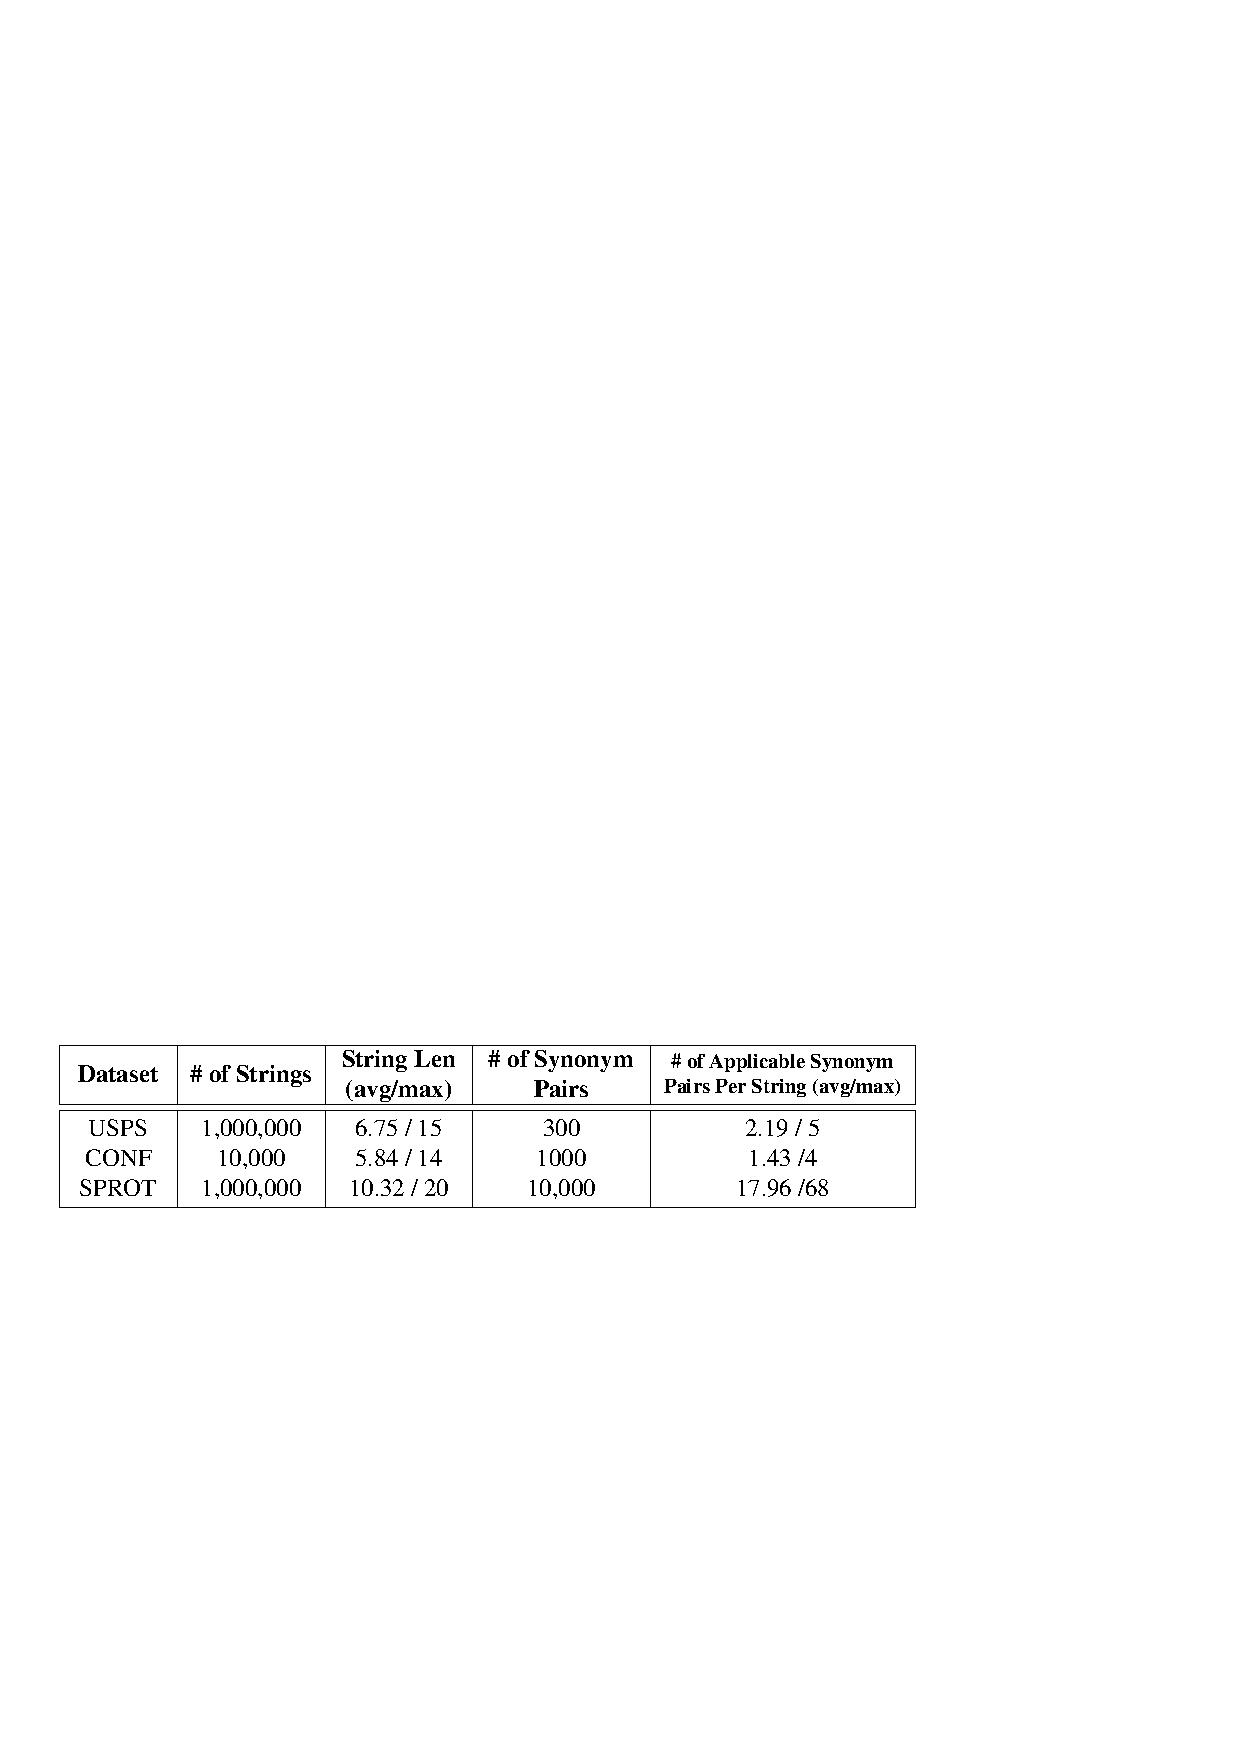
\includegraphics[width=\linewidth]{figures/Characteristics_Datasets}
   \vspace{-6mm}
  \caption{Characteristics of Datasets.}
  \label{tab:data_characteristics}
\end{figure}


Figure~\ref{tab:data_characteristics} gives the characteristics of the
three datasets.

\subsection{Effectiveness of taxonomy for string joins}

The first experiment is to demonstrate the effectiveness of
taxonomy for string joins. We compared our
two measures: Jaccard similarity, full expansion
  (\textbf{Full}), and  our similarity with taxonomy.

For each of the three datasets, we performed the experiments by conducting a similarity join between the
query table $T_Q$ and the target table $T_T$ as follows: (1) $T_Q$ consists of 100 manually selected
full names, and (2) $T_T$ has 500 records where 100 of them
are the correct abbreviations of the corresponding records in $T_Q$
(i.e., the ground truth), and the other 400 random records are selected from string collections. This is to
ensure that there is only one correct matching record in $T_T$ for each
 record in $T_Q$.

Quality of Measures.

In Figure \ref{fig:quality}, we report the quality of the measures by testing the \textit{Precision} (short for ``P''),  \textit{Recall} (``R''), and \textit{F-measure$=\frac{2\times P \times R}{P+R}$} (``F'') on three datasets. We observe that:

\noindent$\bullet$ The similarity measures using synonyms (including \textit{JaccT}, \textit{Full} and \textit{SE}) obtain higher scores than Jaccard which does not consider synonym pairs. The reason is that without using synonyms, Jaccard has no chance to improve the similarity.

%\noindent$\bullet$  \textit{Full} achieves a comparable performance with \textit{JaccT}. Note that \textit{JaccT}  selects only appropriate synonyms to increase the similarity, but \textit{Full} utilizes all the applicable rules and most rules in \textit{Full} is useful, since it is not common that synonyms contain ambiguous meanings. In addition, note hat \textit{Full} is much more efficient than \textit{JaccT}, which will be demonstrated later.


\noindent$\bullet$ \textit{SE} significantly outperforms \textit{JaccT} in each dataset. For example, on SPROT dataset, the F-measures of \textit{SE} and \textit{JaccT} are $0.82$ and $0.52$, respectively. The main reason is that: an abbreviation may have various full expressions and the join records may contain the combination of multiple expressions. Therefore \textit{SE} can apply multiple rules, while \textit{JaccT} can apply only one. Note that such situation is not rare in the real world, as one fragment of a string likely involves multiple synonym rules. We illustrate one example on each of three datasets in Figure \ref{fig:quality} to compare the performance of four similarity measures. For example, see CONF data in Figure \ref{fig:quality}, ``\textsf{VLDB}'' has two different full expressions, i.e., ``\textsf{International Conference on Very Large Databases}'' ($r_1$) and ``\textsf{Proceedings of the VLDB Endowment}''($r_2$), and $s1$ contains these two expressions.  \textit{SE} applies both $r_1$ and $r_2$ to $s_2$ to obtain a high similarity score, i.e., 0.93, while \textit{JaccT} can only apply $r_2$ to $s_2$ and the similarity is only $0.57$. Assume that the join threshold is 0.8, then  \textit{JaccT} can not find the correct answer while \textit{SE} can.

\subsection{Efficiency and scalability of exact-join algorithms}

The second set of experiments is to test the efficiency and scalability of
various exact-joins algorithms. We compared our algorithms, the \textbf{baseline}
and \textbf{TIndex}.

Metrics.

 We took the following measures: (i) the running time (including filtering time, verification time and the time for building QP-tree for a query), and (ii) the size of candidates.

Running Time and Scalability.
Figure~\ref{fig:search_scalability_datasize} shows the running time of the four search algorithms, where the threshold is $0.9$. As shown, the running times of Search-baseline(F) and Search-baseline(S) have an exponential growth, whereas QP-search(F) and QP-search(S) scale better (i.e., linear). The reason is that QP-search generates less candidates for the final verification.

To study the scalability of algorithms with the various threshold values, we plotted Figure \ref{fig:search_scalability_threshold}. As shown, the running time of the algorithms decreases with the growth of the threshold values. In addition,  QP-search scales well with various thresholds. In contrast, when the threshold value is small, the running time of Search-baseline increases significantly. For example, in Figure \ref{fig:search_scalability_threshold}(b), when threshold=0.9, the running time of Search-baseline is about 7 times more than that of QP-search. In addition, when the threshold=0.5, the performance of QP-search is at least 15 times better than Search-baseline.

We then study the time cost of Search-baseline and QP-search with different number of synonyms. Recall that the similarity search proceeds to  generate signatures (or QP-index) for a given query, and then to filter the candidates by checking the overlaps of the signatures, and finally to verify the similarity. Therefore, we reported the individual execution time of signature-generation, filtering and verification in Figure  \ref{fig:search_synonyms_conf}. As seen from this figure, we observe that QP-Search(S) significantly outperforms Search-baseline(S) by one order of magnitude. The main reasons are as follows:



(i)  Search-baseline(S) needs to union all the signatures computed from each possible expanded set, while QP-Search(S) directly utilizes the intermediate signatures. Therefore, the time of signature-generation of QP-Search(S) is less than that of Search-baseline(S).

(ii) For the filtering phase, QP-Search(S) utilizes the SI-Index and QP-index to achieve stronger filtering power than Search-baseline(S). Thus, the filtering time of QP-Search(S) is less than Search-baseline(S). In addition, due to the powerful filtering, QP-Search(S) generates less candidates than that of Search-baseline(S). For example, in Figure  \ref{fig:search_synonyms_conf}, we reported the number of candidates for each query. As shown, the number of candidates of Search-baseline(S) is about one order of magnitude more than that of QP-search(S).

(iii)  QP-Search(S) spends less time on verifying the candidates than Search-baseline(S). Therefore, the verification time of QP-Search(S) is less than that of Search-baseline(S).

Therefore, QP-Search(S) outperforms Search-baseline(S) in each of the three phases.  Experiments in USPS and SPROT datasets have the similar trend (as shown in Figure \ref{fig:search_synonyms_usps} and Figure \ref{fig:search_synonyms_sprot}, respectively).

\subsection{Efficiency and scalability of approximate-join algorithms}

The third set of experiments is to test the efficiency and scalability of
approximate-join algorithms. We compared the algorithms \textbf{baseline}
and \textbf{SI-Join}.  We implemented all algorithms using both
prefix and LSH filters. Therefore, with respect to the algorithms using
LSH scheme, we append ``-LSH'' to the name, e.g., JaccT-LSH denotes the
JaccT algorithm using LSH scheme. Note that, we use the false negative
ratio $\delta \leq 5\%$, i.e., the accuracy is $1-\delta \geq 95\%$. The
parameters $k$ and $l$ should satisfy: $\delta \geq
(1-\theta^k)^l$~\cite{journals/tods/XiaoWLYW11}. For example, if
threshold $\theta=0.8$, $k=3$, then $l$ should be at least $5$ to
guarantee $> 95\%$ accuracy.

Metrics. We took the following measures: (i) the size of signatures, (ii) the filtering ratio of the algorithms, which is typically defined as the number~of~pruned~string~pairs divided by the total number of string pairs; and (iii) the running time (including filtering time and verification time).

Number of Signatures.


We first performed experiments to report the number of signatures of a
query string. It has a major impact on the query time, as both \textit{JaccT} and
our join algorithms need to frequently check the overlaps of string
signatures. The results are reported in Figure~\ref{fig:signature-size}.
For both prefix and LSH schemes, the number of signatures of our
expansion-based algorithms is smaller than that of \textit{JaccT}. The reason is
that based on a transformation framework, \textit{JaccT} is more likely to
include new tokens into signatures than ours. In addition, we observe
that the size of signatures in the LSH scheme is greater than that in
prefix scheme, and the gap increases when the threshold decreases. As we
will see shortly, this results in substantial overhead of filtering time
for the LSH scheme.


\textbf{Filtering Power.}

We investigated the filtering power of different algorithms in
Figures~\ref{fig:filter_ratio_prefix} and \ref{fig:filter_ratio_LSH} using
prefix and LSH schemes, respectively. The experiments were performed on
USPS and SPROT datasets for self-join. For prefix-based algorithms,
Join-baseline is slightly better than JaccT, while SI-Join has a substantial
lead over JaccT and Join-baseline. These results are mainly because of the
additional filtering power in SI-Join brought by length filtering and
signature filtering. Next, for LSH-based algorithms, Figure
\ref{fig:filter_ratio_LSH} demonstrates the similar trend. That is,
SI-Join is the winner in all settings by varying the parameters $k$ and
$l$. Compared to the prefix scheme, LSH has a slightly higher filtering
ratio when parameters are set optimally (e.g. 99.2\% v.s. 98.9\% in USPS
data, with threshold 0.9). On the other hand, note that LSH may filter
away correct answers, resulting in false negatives, as can be seen from
the false negative percentages shown in
Figure~\ref{fig:filter_ratio_LSH}.

\textbf{Effects of different filters.}

We analyzed the effects of different filters, i.e., signature-filters, length-filters and  signature-plus-length. As shown in Figure \ref{fig:filter_methods},  signature-plus-length filters obtain the strongest filtering power on all the datasets, which explains why our algorithms use these two kinds of filters together. There is no absolute winner between signature filters and length filters. In particular, signature filters have stronger filtering power on the USPS dataset (Figure \ref{fig:filter_methods}(a)), while the opposite situation occurs in the SPROT dataset (Figure \ref{fig:filter_methods}(c)), i.e., length filters beat signature filters. On the CONF dataset (Figure \ref{fig:filter_methods}(b)), when the threshold value is small, signature filters win length filters. However, when the threshold value is high, length filters beat signature filters. Therefore, the individual effects of signature filters and length filters depend on the data sets and the thresholds, and the combined structure of both (i.e. SI-tree) achieves the best results.


\textbf{Running Time and Scalability.}


Figure~\ref{fig:scalability} and Figure \ref{fig:scalability_LSH} show the running time of five join algorithms based on prefix and LSH schemes, respectively, where the join threshold is $0.8$. The x-axis represents the join data size. As shown, the running times of both JaccT and Join-baseline (i.e., Join-baseline(F), Join-baseline(S)) have an exponential growth, whereas SI-Join (i.e., SI-Join(F), SI-Join(S))  scales better (i.e., linear) than Join-baseline and JaccT. The reason is that SI-Join methods have more efficient filtering strategies and generate smaller size of candidates.  In addition, in order to study the scalability of algorithms with the increase of the number of rules, we plot Figure \ref{fig:synonyms}(b), where  SI-Join(F) (i.e., SI-Join with the full-expansion) is a clear winner in algorithms using rules: it is insensitive to the number of rules and thus able
to outperform other methods when one string involves more than 10 rules.


\smallskip

\noindent \textbf{Summary} ~~ Finally, we summarize the main findings.

(1) Considering four similarity measures, we observe that \textit{Jaccard} is inadequate due to its complete neglect of synonym rules. \textit{JaccT} is not efficient because it enumerates all transformed strings and entails large query overhead. \textit{Full-expansion} is extremely efficient, but its F-measure is not as good as \textit{Selective-expansion}, which makes a good balance between effectiveness and efficiency.

(2)	With respect to the similarity searches and joins,  QP-search and SI-join are the winners in the settings, respectively over the previous algorithms (i.e., \textit{JaccT}) and baseline methods. Note that we achieve a speedup of up to 50$\sim$300x on three data sets over the state-of-the-art approach.

(3) Finally, 2DHS synopsis offers very good results, and is extremely efficient to estimate the filtering power of different filters, ( $<$ 1 second ,  accounting for only 1\% of the total running time),  which strongly motivates its application in practice.



\section{Related work} \label{sec:relatedwork}

Taxonomy is the practice and science of classification. Many taxonomies have a hierarchical structure, but this is not a requirement. In this work, we study to leverage the existing taxonomy to improve the accuracy of string record join in databases. Such a taxonomy could be constructed manually
through experts and community efforts, as in WordNet
[4], Cyc [14], and Freebase. With the advantage of freshness
and informativeness, automatic taxonomy construction has
been extensively studied recently, for example, in [20, 22,
18, 21, 26]. WikiTaxonomy [18] and YAGO [22] may be the
most notable efforts, which attempt to derive a taxonomy
from Wikipedia categories. With more web data, Probase
[26] aims at building a unified taxonomy of worldly facts.

In recent years, we have witnessed the emergence of various efforts to enhance the effectiveness of string similarity joins by using synonyms \cite{conf/sigmod/LuLWLW13,conf/icde/ArasuCK08,conf/cpm/BarbayGMR06,conf/vldb/ArvindSR09}.
The traditional similarity functions consider only syntactic similarities, e.g., number of common
words or $q$-grams. But there are many important cases where syntactically different
strings can represent the same real-world object. For example,
``\textsf{Bill}'' is a short form of ``\textsf{William}'', and ``\textsf{ICDE}'' is an abbreviation of  ``\textsf{International Conference on Data Engineering}''.  Given two collections of strings,  synonym-based similarity functions can utilize the available synonyms to find string pairs which are semantically similar. While those methods improve the effectiveness of string joins, a synonym dictionary does not contain information such as
``\textsf{Helsinki is the capital of Finland}'', or `\textsf{`Apple 6 Plus is a new model of iPhone}''. Still, term pairs such as ``\textsf{Helsinki}'' and ``\textsf{Finland}'', ``\textsf{Apple 6 Plus}'' and ``\textsf{iPhone}''  have strong semantic correlations.



Taxonomies are is-a hierarchies of concepts, topics, or keywords. Since they represent ontology specializations, they may be
used to provide meaningful knowledge representations and, thus, support users in understanding the semantic meaning of a
resource and the related domain.
Several efforts to integrate taxonomies in the Data mining and Knowledge Discovery (KDD) process have been done. For
instance, taxonomies have already been exploited to (i) discover high level correlations among data [9�C13], (ii) perform textual
data analysis and summarization [14,15,35,36], (iii) improve user browsing by looking into the results of Web search engines
[37], and (iv) enhance the quality of recommendation systems [17,38]. This paper focuses on exploiting taxonomy information to
enrich data used for classification. To the best of our knowledge, it is the first attempt to integrate high level and multi-faceted
knowledge into classifier construction.


Several types of Similarity Join have been proposed in the
literature, e.g., distance range join (retrieves all pairs whose distances
are smaller than a predefined threshold $\varepsilon$) [2, 3, 4, 5, 6,
7], k-Distance join (retrieves the k most-similar pairs) [8], and
kNN-join (retrieves, for each tuple in one table, the k nearest neighbors
in another table) [9, 10, 11]. The distance range join
has been one of the most studied and useful types of Similarity
Join. This type of join is commonly referred to simply as Similarity
Join and is the focus of this paper. Among its most relevant
implementation techniques, we find approaches that rely
on the use of pre-built indices, e.g., eD-index [3], D-index [4],
and List of Twin Clusters (LTC) [12]. These techniques strive
to partition the data while clustering together the similar objects.
While these indexing techniques support the SJ operation
they also have some shortcomings: D-index and eD-index may
require rebuilding the index to support queries with different $\varepsilon$,

Approximate string matching includes finding (sub)strings
that resemble a given query string. It is a well-researched
topic and has many applications, such as data cleansing [1],
spelling correction [19], query autocompletion [33], near duplicate
detection [25, 32], approximate named entity recognition
[29], and bioinformatics [20, 27, 35].
Due to the sheer amount of literature in this area, we will
focus on most related recent results and refer readers to the
excellent surveys [13, 22] and tutorials [3, 12, 16] for a comprehensive
treatment of the topic.
Based on the types of the queries, recent work focuses either
on efficient single query processing (typically named string
similarity queries) [1, 6, 9, 11, 18, 25, 28, 31], or the similarity
join which can be treated as processing a batch of similarity
queries [2, 8, 10, 12, 14, 17, 28, 29, 34, 35]. Most recently,
Jiang et al. [15] experimentally evaluate and analyze many of
the existing similarity join algorithms.


$\mathbf{Prefix filter.}$ Since the prefix
filter is effective, many methods are proposed to optimize it
for different similarity operators. ED-
join [12,28] proposed a location-based mismatch filter to re-
duce prefix length and a content-based mismatch filter to
reduce the number of candidates for ED. Pivotal prefix filter [4] reduced the prex length for ED. PassJoin [17] pro-
posed segment filter to improve pruning power. PPJoin [29]
used the positions of prefix and suffix to improve pruning
power for token-based similarities. Length filter was pro-
posed to prune dissimilar answers based on length difference [8]. TrieJoin [23] used a different framework that directly computed real similarity using the trie structure.





\section{Conclusion}

In this paper, we presented a framework which use the exsting taxonomy to perform exact and approximate.
concepts included.

We introduce a new query type, approximate string join, with taxonomy. We propose processing
models for taxonomy queries, and introduce how to build
an additional index (besides the inverted index) to support
efficient query processing. In particular, we study the problem
of how to optimize this additional index based on a
workload of queries, with the goal of minimizing query processing
cost, and propose algorithms with performance guarantees.
Our index optimization techniques are tested using
real datasets and are shown to be effective and robust.


\bibliographystyle{abbrv}
\bibliography{localrefs}



\end{document}
